\chapter{Resultados Parciais}
\label{chap:resultadosparciais}

	Em vista dos procedimentos teóricos aliados a uma solução computacional, obteve-se 3 tipos de resultados sequênciais de processamento de áudio.
	Cada um dos resultados depende de seu anterior não podendo, por consequência, obter um resultado satisfatório no último procedimento sem ter êxito nos anteriores. Os 3 tipos de resultados são:
	 \begin{itemize}
        \item resultado da resposta em frequência;
        \item resultado da sugestão de notas;
        \item resultado da sugestão de acordes.
    \end{itemize}

\section{Resultado da Resposta em Frequência}
\label{sec:resultadodarespostaemfrequencia}

A primeira camada de processamento da solução computacional proposta é a relativa a transformada de fourier. O resultado dessa camada é um vetor de 22.000 posições. Cada posição referente a frequência e sua resposta o valor da mesma.
Segue o gráfico resultante:

 \begin{figure}[h]
	\centering
		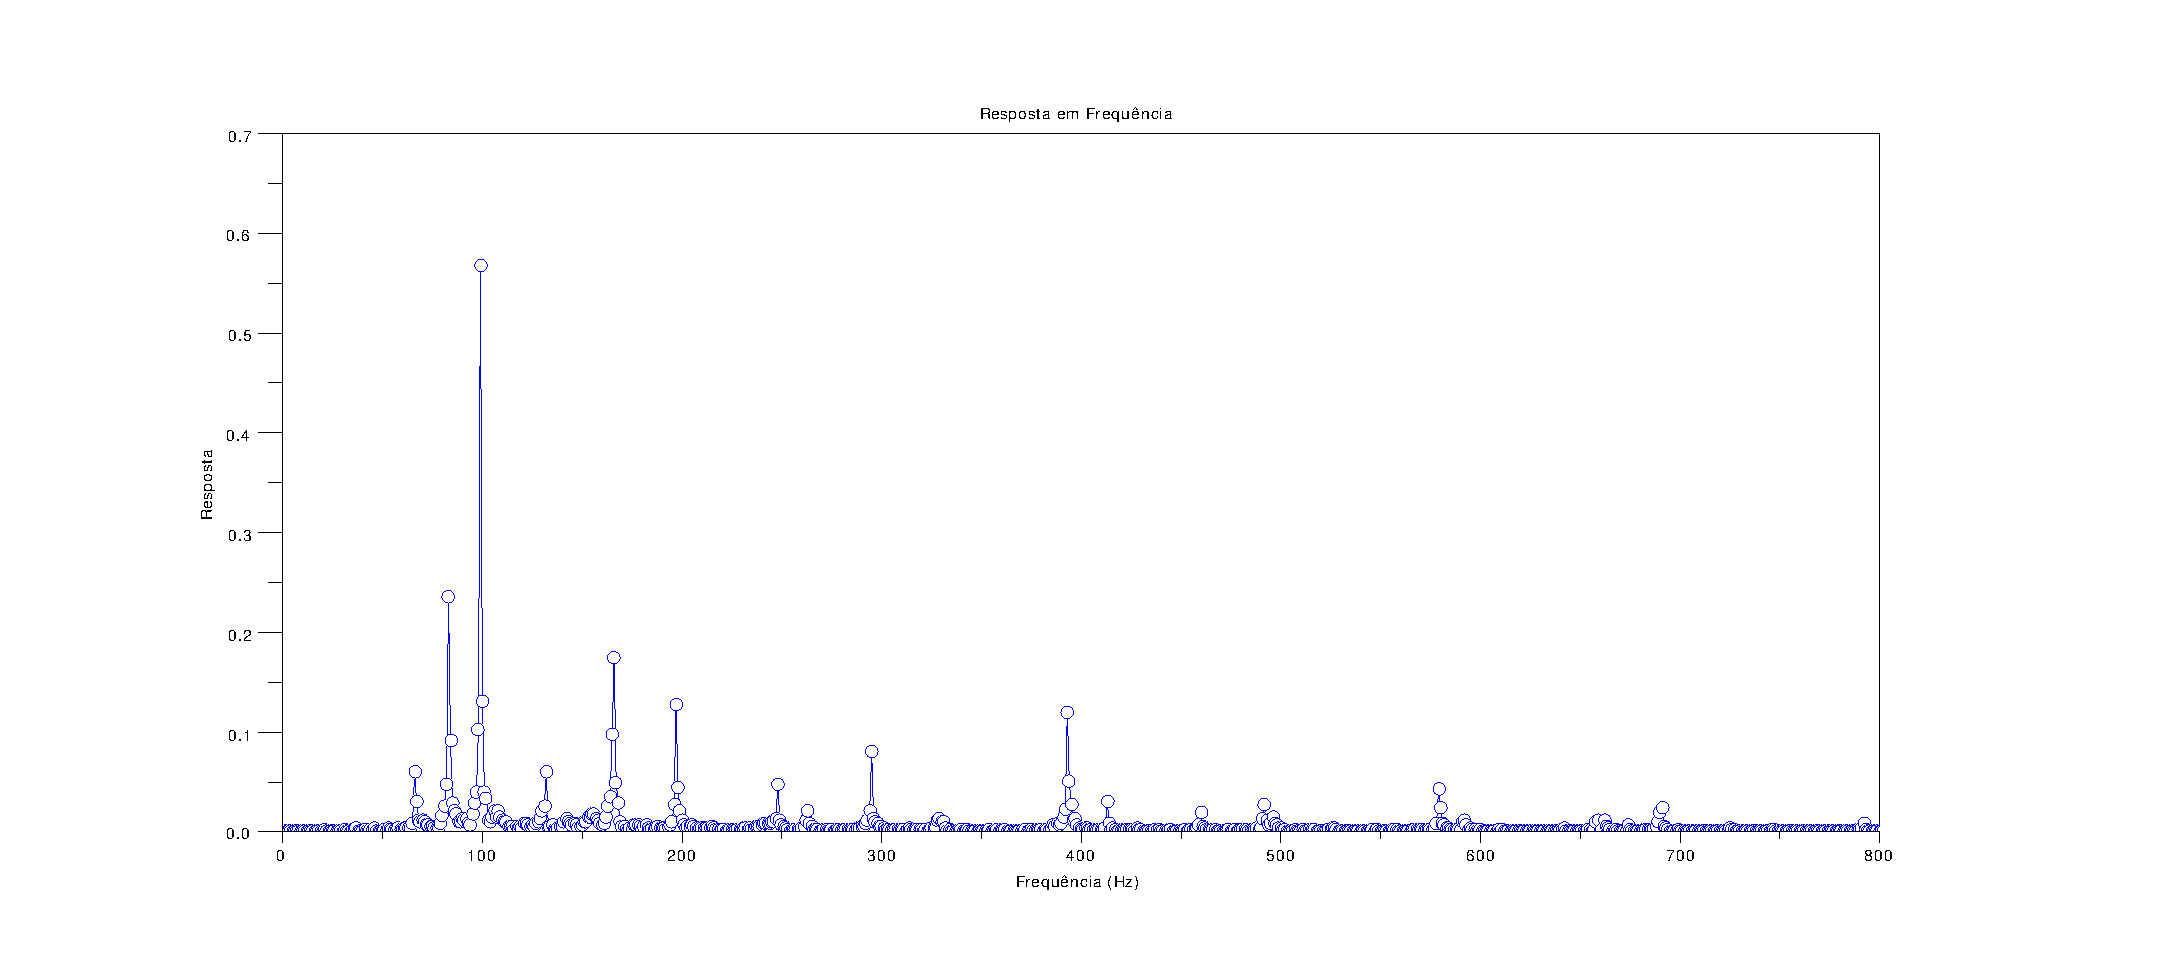
\includegraphics[keepaspectratio=true,scale=0.49]{figuras/resposta_frequencia.eps}
	\caption{Gráfico da resposta em frequência do arquivo de áudio processado}
\end{figure}

Nesse gráfico é possível perceber os 3 primeiros picos que identificam a natureza da composição do sinal. O primieiro pico, no valor de 66 Hz, é relativo ao dó2. O segundo pico, no valor de 83 Hz, é relativo ao mi2. O terceiro pico, no valor de 99 Hz, é relativo ao sol2. 

Analisando o gráfico é possível inferir que ele caracteriza acorde dó maior devido a presença de alta energia da tríade relatada. Um fato interessante é que os outros picos que se seguem são relativos aos harmônicos das notas e não descaracterizam o acorde, mas, pelo contrário, enfatizam o perfil harmônico do sinal de áudio.

\section{Resultado da Sugestão de Notas}
\label{sec:resultadodasugestaodenotas}

A segunda camada é a da rede neural para sugestão de notas. Ela tem como insumo de entrada a transformada de fourier. O resultado dessa camada é um vetor de 12 posições. Cada posição é representada por uma nota musical. Segue o gráfico resultante: 

\begin{figure}[h]
	\centering
		\includegraphics[keepaspectratio=true,scale=0.49]{figuras/notas.eps}
	\caption{Gráfico de sugestão de notas do arquivo de áudio processado}
\end{figure}

Ao visualizar o gráfico é possível perceber que as notas sol, mi, sol\#
 e dó são as que possuem mais energia ou, no ponto de vista de sugestão, as mais sugeridas. Mesmo pela alta sugestão da nota sol\#
 que é oriunda de erros de arredondamento, de certa forma essa combinação caracteriza o acorde dó maior.   

%\newpage
\section{Resultado da Sugestão de Acordes}
\label{sec:resultadodasugestaodeacordes}

A terceira camada é a da rede neural para sugestão de acordes. Ela tem como insumo de entrada as sugestões de notas da rede neural anterior. O resultado dessa camada é um vetor de 48 posições. Cada posição é representada por um tipo de acorde diferente entre as possibilidades de acorde maior, menor, aumento e diminuto para cada nota musical. Segue os gráficos resultantes:

\begin{figure}[h]
	\centering
		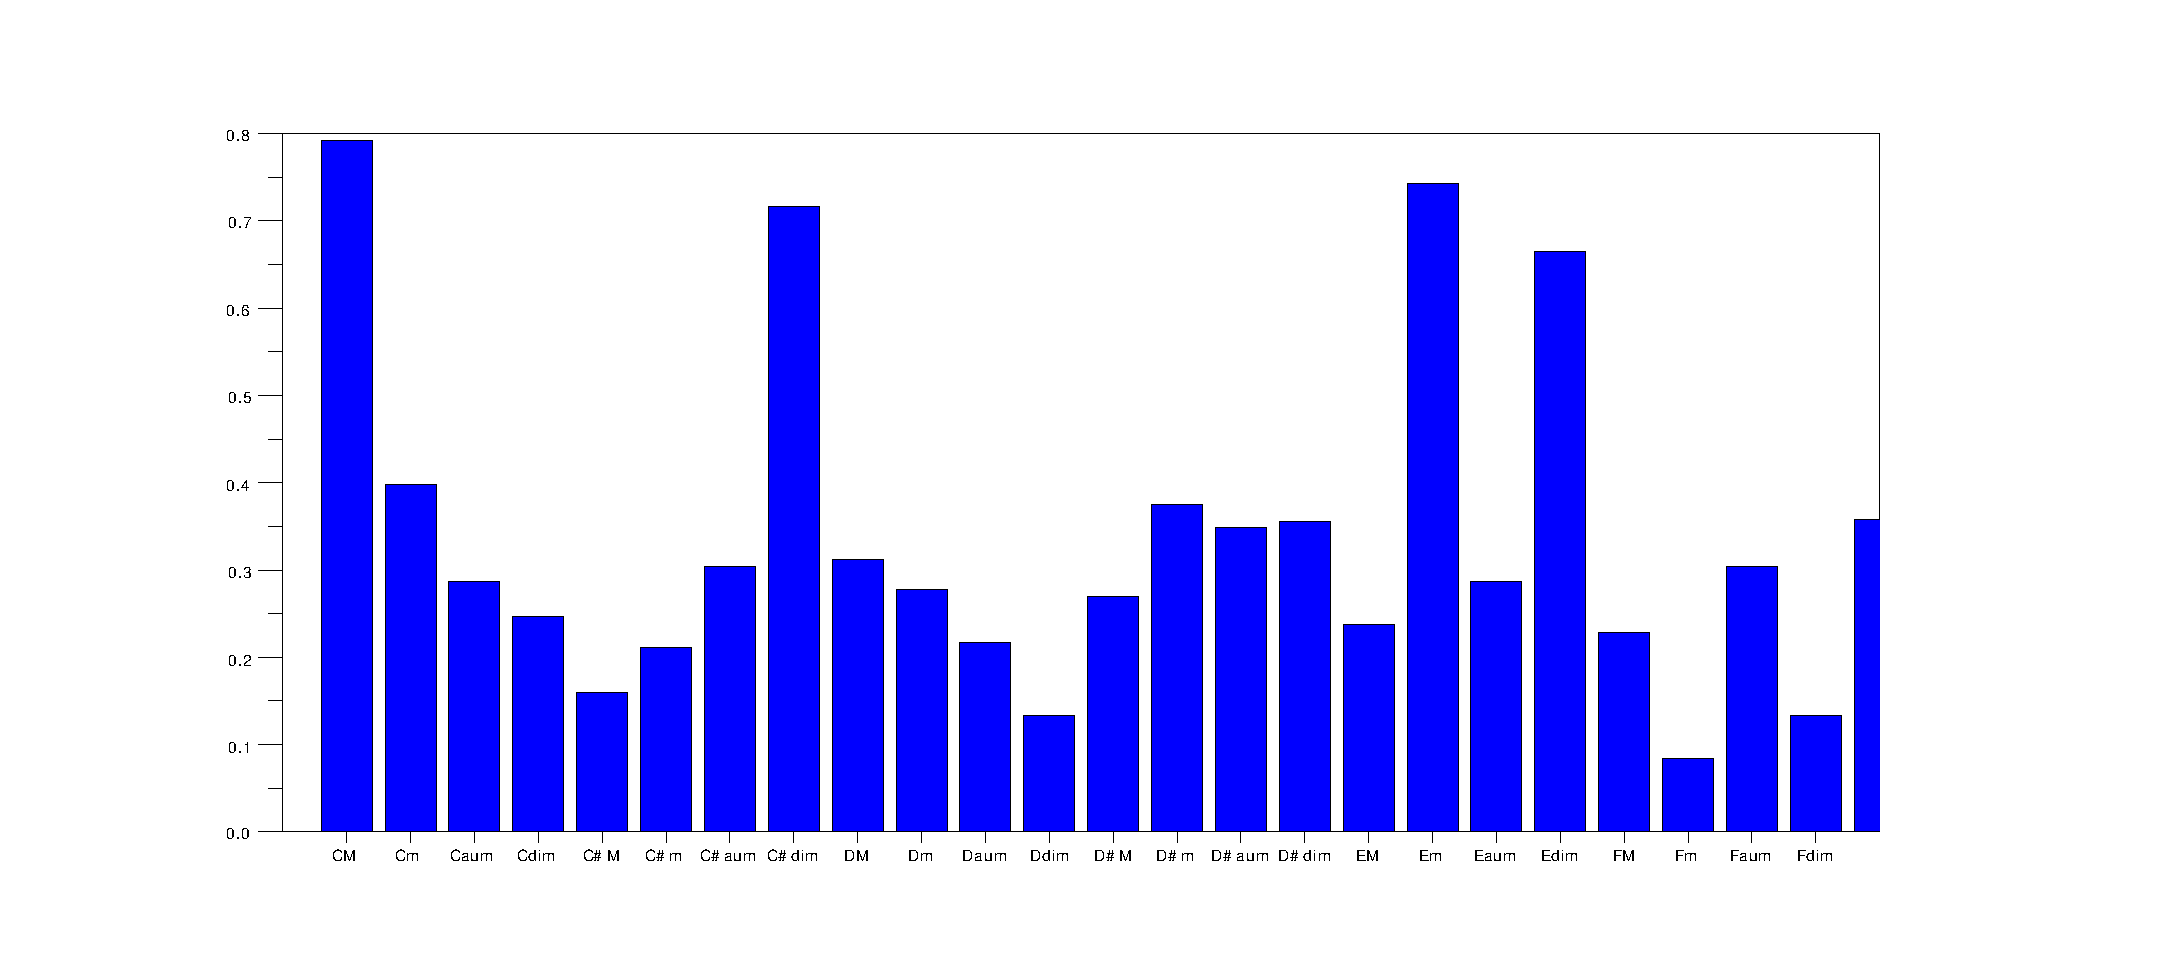
\includegraphics[keepaspectratio=true,scale=0.49]{figuras/sugestaoacordes1.eps}
		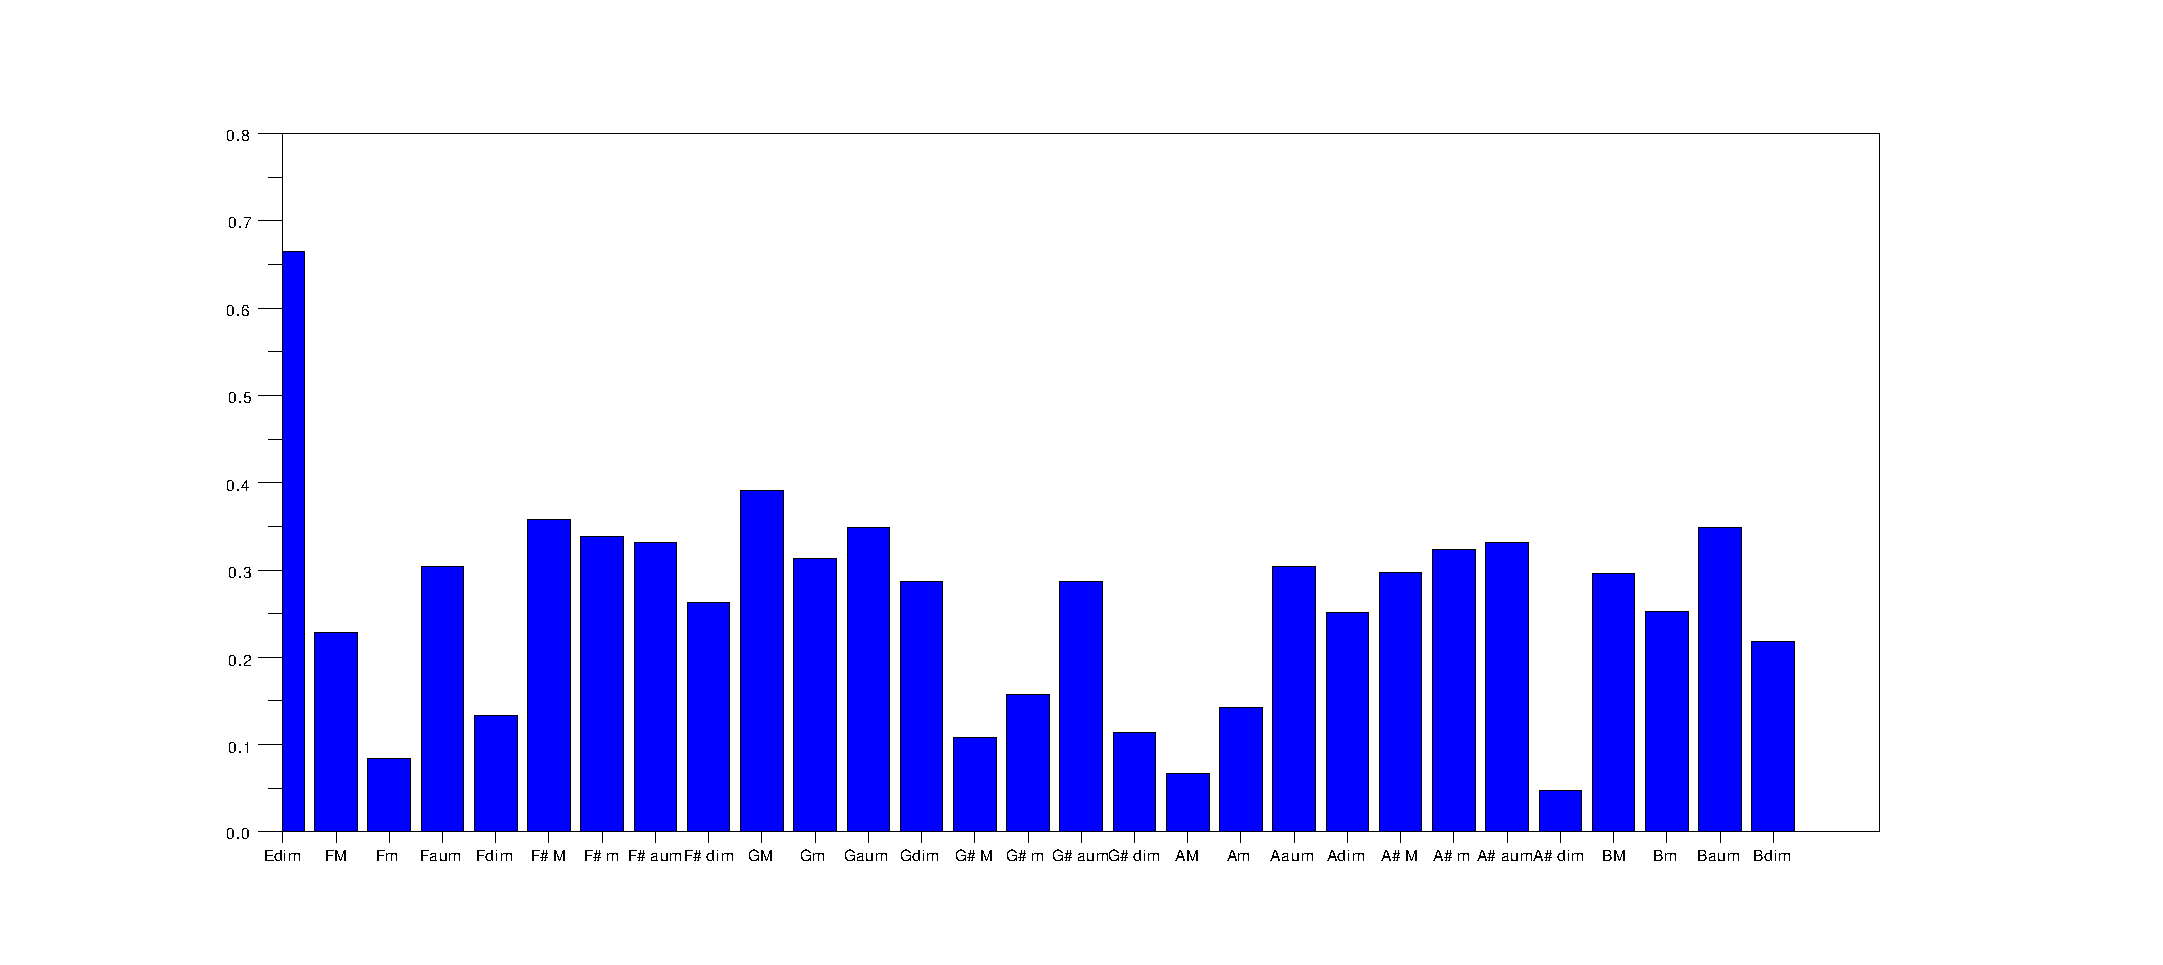
\includegraphics[keepaspectratio=true,scale=0.49]{figuras/sugestaoacordes2.eps}
	\caption{Gráficos de sugestão de acordes do arquivo de áudio processado}
\end{figure}

Analisando esses dois gráficos é perceptível a presença do acorde CM ou dó maior para a maior sugestão. Logo, o sistema classifica o arquivo de áudio processado como acorde de dó maior.